\documentclass[10pt]{beamer}

\mode<presentation>{% Settings
    % link to view http://www.hartwork.org/beamer-theme-matrix/
    % ------------------------------------------------------------------------------
    % Slide Themes
    % ------------------------------------------------------------------------------
    % \usetheme{default}
    % \usetheme{AnnArbor}
    % \usetheme{Antibes}
    % \usetheme{Bergen}
    % \usetheme{Berkeley}
    \usetheme{Berlin}
    %\usetheme{Boadilla}
    %\usetheme{CambridgeUS}
    %\usetheme{Copenhagen}
    %\usetheme{Darmstadt}
    %\usetheme{Dresden}
    %\usetheme{Frankfurt}
    %\usetheme{Goettingen}
    %\usetheme{Hannover}
    %\usetheme{Ilmenau}
    %\usetheme{JuanLesPins} % rounded title, gradient at top with section, no bottom bar
    % \usetheme{Luebeck}     % square title, toc at top of each slide
    %\usetheme{Madrid}      % rounded title
    %\usetheme{Malmoe}
    %\usetheme{Marburg}
    %\usetheme{Montpellier}
    % \usetheme{PaloAlto}
    %\usetheme{Pittsburgh}
    %\usetheme{Rochester}
    %\usetheme{Singapore}
    %\usetheme{Szeged}
    %\usetheme{Warsaw}

    % ------------------------------------------------------------------------------
    % Color Schemes
    % ------------------------------------------------------------------------------
    %\usecolortheme{default}
    %\usecolortheme{albatross}  % blue background with darker blue
    %\usecolortheme{beaver}     % gray with red
    %\usecolortheme{beetle}     % gray background
    %\usecolortheme{crane}      % orange
    \usecolortheme{dolphin}     % white with purple
    %\usecolortheme{dove}       % all white
    %\usecolortheme{fly}        % all gray including background
    %\usecolortheme{lily}       % white with blue
    %\usecolortheme{orchid}     % default blue
    %\usecolortheme{rose}       % default blue
    %\usecolortheme{seagull}    % darker gray than seahorse
    %\usecolortheme{seahorse}   % light gray blueish tint
    %\usecolortheme{whale}      % default blue
    %\usecolortheme{wolverine}  % yellow with a little blue

    %\setbeamertemplate{footline} % To remove the footer line in all slides uncomment this line
    %\setbeamertemplate{footline}[page number] % To replace the footer line in all slides with a simple slide count uncomment this line
    \setbeamertemplate{navigation symbols}{} % To remove the navigation symbols from the bottom of all slides uncomment this line
    \setbeamertemplate{bibliography item}{\insertbiblabel} % to number bibliography entries
}

\usepackage{Logemann}
\usepackage{Integral}
\usepackage{LinearAlgebra}
\usepackage{Derivative}
\usepackage{Vector}
\usepackage{Sum}
\usepackage{SetTheory}
\usepackage{booktabs}
\usepackage[backend=biber]{biblatex}
\addbibresource{refs.bib}

\title[]{Nonconservative Discontinuous Galerkin Method for Generalized Shallow Water Equations} % The short title
% appears at the bottom of every slide, the full title is only on the title page

\author{Caleb Logemann \and James Rossmanith} % Your name
\institute[Iowa State University]{% Your institution as it will appear on the bottom of every slide, may be shorthand to save space
Mathematics Department,\\ Iowa State University \\ % Your institution for the title page
\medskip
\textit{logemann@iastate.edu}} % Your email address

\date{March 05, 2021} % Date, can be changed to a custom date

\begin{document}
  \begin{frame}
    \titlepage{}
  \end{frame}

  \begin{frame}
    \frametitle{Overview}
    \tableofcontents
  \end{frame}

  \section{Generalized Shallow Water Equations}
    \begin{frame}
      \frametitle{Generalized Shallow Water, (\textcite{kowalski2017moment})}
      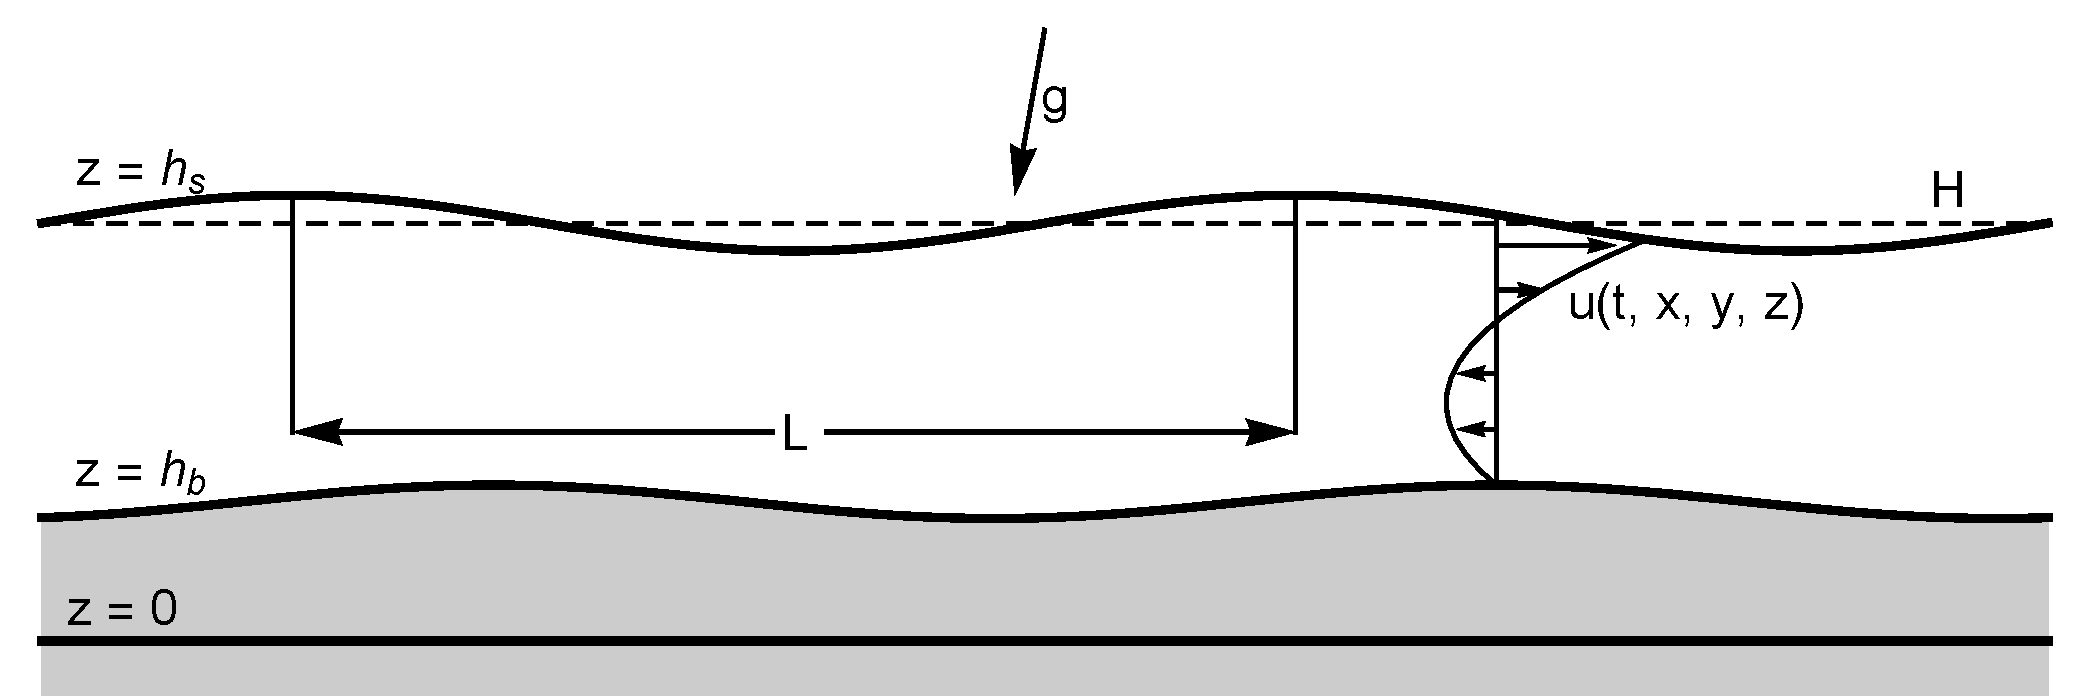
\includegraphics[scale=0.28]{Figures/ShallowWaterModel.pdf} \\
      Incompressible Navier Stokes Equations with a free surface
      \begin{align*}
        \div{\v{u}} &= 0 \\
        \v{u}_t + \div*{\v{u}\v{u}} &= - \frac{1}{\rho} \grad{p}
        + \frac{1}{\rho} \div{\sigma} + \v{g}
      \end{align*}
      \begin{align*}
        \p{h_s}_t + \br{u(t, x, y, h_s), v(t, x, y, h_s)}^T \cdot \grad{h_s}
        &= w(t, x, y, h_s) \\
        \p{h_b}_t + \br{u(t, x, y, h_b), v(t, x, y, h_b)}^T \cdot \grad{h_b}
        &= w(t, x, y, h_b)
      \end{align*}
    \end{frame}

    \begin{frame}
      \frametitle{Polynomial Ansatz}
      \begin{align*}
        \tilde{u}(t, x, y, \zeta) &= u_m(t, x, y) + u_d(t, x, y, \zeta) \\
        &= u_m(t, x, y) + \sum{j = 1}{N}{\alpha_j(t, x, y) \phi_j(\zeta)} \\
        % &= \sum{j = 0}{N}{\alpha_j(t, x, y) \phi_j(\zeta)} \\
        \tilde{v}(t, x, y, \zeta) &= v_m(t, x, y) + v_d(t, x, y, \zeta) \\
        &= v_m(t, x, y) + \sum{j = 1}{N}{\beta_j(t, x, y) \phi_j(\zeta)}
        % &= \sum{j = 0}{N}{\beta_j(t, x, y) \phi_j(\zeta)}
      \end{align*}
      Orthogonality Condition
      \[
        \dintt{0}{1}{\phi_j(\zeta) \phi_i(\zeta)}{\zeta} = 0 \quad \text{for } j \neq i
      \]
      \begin{align*}
        \phi_0(\zeta) = 1, \quad
        \phi_1(\zeta) = 1 - 2\zeta, \quad
        \phi_2(\zeta) = 1 - 6\zeta + 6 \zeta^2
        % &\phi_3(\zeta) = 1 - 12\zeta + 30\zeta^2 - 20\zeta^3
      \end{align*}
    \end{frame}

    \begin{frame}
      \frametitle{Constant Moments}
      Continuity Equation
      \begin{gather*}
        h_t + \p{hu_m}_x + \p{hv_m}_y = 0
        \intertext{Conservation of Momentum Equations}
        \p{h u_m}_t
        + \p{h\p{u_m^2 + \sum*{j = 1}{N}{\frac{\alpha_j^2}{2j + 1}}} + \frac{1}{2}g e_z h^2}_x \\
        + \p{h\p{u_m v_m + \sum*{j = 1}{N}{\frac{\alpha_j \beta_j}{2j + 1}}}}_y
        = -\frac{\nu}{\lambda} \p{u_m + \sum*{j = 1}{N}{\alpha_j}} + hg\p{e_x - e_z\p{h_b}_x} \\
        \p{h v_m}_t
        + \p{h\p{v_m^2 + \sum*{j = 1}{N}{\frac{\alpha_j \beta_j}{2j + 1}}} + \frac{1}{2}g e_z h^2}_y \\
        + \p{h\p{u_m v_m + \sum*{j = 1}{N}{\frac{\alpha_j \beta_j}{2j + 1}}}}_x
        = -\frac{\nu}{\lambda} \p{v_m + \sum*{j = 1}{N}{\beta_j}} + hg\p{e_y - e_z\p{h_b}_y}
      \end{gather*}
    \end{frame}

    \begin{frame}
      \frametitle{Higher Order Moments}
      % Moment Equations
      \small
      \begin{gather*}
        \p{h\alpha_i}_t + \p{2 h u_m \alpha_i + h\sum*{j,k=1}{N}{A_{ijk}\alpha_j \alpha_k}}_x
        + \p{h u_m \beta_i + h v_m \alpha_i + h\sum*{j,k=1}{N}{A_{ijk}\alpha_j \beta_k}}_y \\
        = u_m D_i - \sum*{j,k=1}{N}{B_{ijk}D_j \alpha_k} - \p{2i + 1} \frac{\nu}{\lambda} \p{u_m + \sum*{j=1}{N}{\p{1 + \frac{\lambda}{h}C_{ij}}\alpha_j}} \\
        \p{h\beta_i}_t + \p{h u_m \beta_i + h v_m \alpha_i + h\sum*{j,k=1}{N}{A_{ijk}\alpha_j \beta_k}}_x
        + \p{2 h v_m \beta_i + h\sum*{j,k=1}{N}{A_{ijk}\beta_j \beta_k}}_y \\
        = v_m D_i - \sum*{j,k=1}{N}{B_{ijk}D_j \beta_k} - \p{2i + 1} \frac{\nu}{\lambda} \p{v_m + \sum*{j=1}{N}{\p{1 + \frac{\lambda}{h}C_{ij}}\beta_j}}
      \end{gather*}
    \end{frame}

    \begin{frame}
      \frametitle{Example Systems}
      1D model with \(h_b\) constant, \(e_x = e_y = 0\), and \(e_z = 1\) \\
      Constant System
      \begin{align*}
        \begin{bmatrix}
          h \\
          h u_m
        \end{bmatrix}_t +
        \begin{bmatrix}
          h u_m \\
          h u_m^2 + \frac{1}{2} g h^2
        \end{bmatrix}_x =
        -\frac{\nu}{\lambda}
        \begin{bmatrix}
          0 \\
          u_m
        \end{bmatrix}
      \end{align*}
      Flux Jacobian Eigenvalues, \(u_m \pm \sqrt{gh}\)

      Linear System, \(\tilde{u} = u_m + \alpha_1 \phi_1\)
      \begin{align*}
        \begin{bmatrix}
          h \\
          hu_m \\
          h \alpha_1
        \end{bmatrix}_t +
        \begin{bmatrix}
          h u_m \\
          h u_m^2 + \frac{1}{2} gh^2 + \frac{1}{3}h \alpha_1^2 \\
          2 h u_m \alpha_1
        \end{bmatrix}_x = Q
        \begin{bmatrix}
          h \\
          hu_m \\
          h \alpha_1
        \end{bmatrix}_x - \v{s}
      \end{align*}
      \begin{align*}
        Q =
        \begin{bmatrix}
          0 & 0 & 0 \\
          0 & 0 & 0 \\
          0 & 0 & u_m
        \end{bmatrix} \quad
        \v{s} = \frac{\nu}{\lambda}
        \begin{bmatrix}
          0 \\
          u_m + \alpha_1 \\
          3(u_m + \alpha_1 + 4\frac{\lambda}{h} \alpha_1)
        \end{bmatrix}
      \end{align*}
      Quasilinear Matrix Eigenvalues, \(u_m \pm \sqrt{gh + \alpha_1^2}, u_m\)
    \end{frame}

    \begin{frame}
      \frametitle{Example Systems}
      1 dimensional with \(h_b\) constant, \(e_x = e_y = 0\), and \(e_z = 1\) \\
      Quadratic Vertical Profile, \(\tilde{u} = u + \alpha_1 \phi_1 + \alpha_2 \phi_2\)
      \begin{align*}
        \begin{bmatrix}
          h \\
          hu \\
          h \alpha_1 \\
          h \alpha_2
        \end{bmatrix}_t +
        \begin{bmatrix}
          hu \\
          hu^2 + \frac{1}{2} gh^2 + \frac{1}{3}h \alpha_1^2 + \frac{1}{5} h \alpha_2^2 \\
          2hu \alpha_1 + \frac{4}{5}h \alpha_1 \alpha_2 \\
          2hu \alpha_2 + \frac{2}{3}h \alpha_1^2 + \frac{2}{7}h \alpha_2^2
        \end{bmatrix}_x =
        Q
        \begin{bmatrix}
          h \\
          hu \\
          h \alpha_1 \\
          h \alpha_2
        \end{bmatrix}_x - \v{s}
      \end{align*}
      \begin{gather*}
        Q =
        \begin{bmatrix}
          0 & 0 & 0 & 0 \\
          0 & 0 & 0 & 0 \\
          0 & 0 & u - \frac{\alpha_2}{5} & \frac{\alpha_1}{5} \\
          0 & 0 & \alpha_1 & u + \frac{\alpha_2}{7} \\
        \end{bmatrix},
        P = \frac{\nu}{\lambda}
        \begin{bmatrix}
          0 \\
          u + \alpha_1 + \alpha_2 \\
          3\p{u + \alpha_1 + \alpha_2 + 4 \frac{\lambda}{h} \alpha_1} \\
          5\p{u + \alpha_1 + \alpha_2 + 12 \frac{\lambda}{h}\alpha_2}
        \end{bmatrix}
      \end{gather*}
      Quasilinear Matrix Eigenvalues, \(u \pm c \sqrt{gh}\)
      % \begin{gather*}
      %   c^4
      %   - \frac{10 \alpha_2}{7} c^3
      %   - \p{1 + \frac{6\alpha_2^2}{35} + \frac{6 \alpha_1^2}{5}}c^2 \\
      %   + \p{\frac{22\alpha_2^3}{35} - \frac{6\alpha_2 \alpha_1^2}{35} + \frac{10\alpha_2}{7}} c
      %   - \frac{\alpha_2^4}{35} - \frac{6\alpha_2^2 \alpha_1^2}{35} - \frac{3\alpha_2^2}{7} + \frac{\alpha_1^4}{5} + \frac{\alpha_1^2}{5} = 0
      % \end{gather*}
    \end{frame}

  \section{Nonconservative Products}
    \begin{frame}
      \frametitle{Nonconservative Products, (\textcite{dal1995definition})}
      Model Equation
      \[
        \v{q}_t + \div{\v{f}\p{\v{q}}} + g_i(\v{q}) \v{q}_{x_i} = \v{s}(\v{q}) \quad
        \text{for } \p{\v{x}, t} \in \Omega \times \br{0, T}
      \]

      Traditionally searching for weak solutions, find \(\v{q}\) such that
      \[
        \dintt{0}{T}{\dintt{\Omega}{}{\p{\v{q}_t + \div{\v{f}\p{\v{q}}} + g_i(\v{q}) \v{q}_{x_i}} v}{\v{x}}}{t} = \dintt{0}{T}{\dintt{\Omega}{}{\v{s}(\v{q}) v}{\v{x}}}{t}
      \]
      for all \(v \in C^1_0(\Omega \times \br{0, T})\)
    \end{frame}

    \begin{frame}
      \frametitle{Regularization Paths}
      Consider Lipschitz continuous paths,
      \(\v{\psi}:\br{0, 1} \times \RR^p \times \RR^p \to \RR^p \), that satisfy the
      following properties.
      \begin{enumerate}
        \item \(\forall \v{q}_L, \v{q}_R \in \RR^p\),
          \(\v{\psi}(0, \v{q}_L, \v{q}_R) = \v{q}_L\) and
          \(\v{\psi}(1, \v{q}_L, \v{q}_R) = \v{q}_R\)
        \item \(\exists k > 0\), \(\forall \v{q}_L, \v{q}_R \in \RR^p\),
          \(\forall s \in \br{0, 1}\), \(\abs{\pd{\v{\psi}}{s}(s, \v{q}_L, \v{q}_R)}
          \le k \abs{\v{q}_L - \v{q}_R}\) elementwise
        \item \(\exists k > 0\), \(\forall \v{q}_L, \v{q}_R, \v{u}_L, \v{u}_R \in \RR^p\),
          \(\forall s \in \br{0, 1}\), elementwise
          \[
            \abs{\pd{\v{\psi}}{s}(s, \v{q}_L, \v{q}_R) - \pd{\v{\psi}}{s}(s, \v{u}_L, \v{u}_R)}
            \le k \p{\abs{\v{q}_L - \v{u}_L} + \abs{\v{q}_R - \v{u}_R}}
          \]
      \end{enumerate}

      Let \(u = u_0 + H(x - x_0) (u_1 - u_0)\), then regularize
      \[
        u^{\varepsilon}(x) =
        \begin{cases}
          u_0 & x < x_0 - \varepsilon \\
          \psi(\frac{x - x_0 + \varepsilon}{2 \varepsilon}, u_0, u_1) & x_0 - \varepsilon < x < x_0 + \varepsilon \\
          u_1 & x > x_0 + \varepsilon
        \end{cases}
      \]

    \end{frame}

    \begin{frame}
      \frametitle{Nonconservative Product Definition}
      Let \(\v{q} \in BV\p{\Omega \to \RR^p}\) and
      \(g \in C^1\p{\RR^p \to \RR^p \times \RR^p}\), then \(\mu \) is a Borel measure.
      \begin{enumerate}
        \item If \(\v{q}\) is continuous on a Borel set \(B \subset \Omega \), then
          \[
            \v{\mu}(B) = \dintt{B}{}{g(\v{q}) \d{\v{q}}{x}}{x}
          \]
        \item If \(\v{q}\) is discontinuous at a point \(x_0 \in \Omega \), then
          \[
            \v{\mu}({x_0}) = \dintt{0}{1}{g(\v{\psi}(s; \v{q}(x_0^-), \v{q}(x_0^+))) \pd{\v{\psi}}{s}(s; \v{q}(x_0^-), \v{q}(x_0^+))}{s}
          \]
      \end{enumerate}
      Define
      \[
        \v{\mu} = \br[\v{\psi}]{g(\v{q}) \d{\v{q}}{x}}
      \]
    \end{frame}

    \begin{frame}
      \frametitle{Nonconservative Products}
      If there exists \(\v{f}(\v{q})\) such that \(\v{f}'(\v{q}) = g(\v{q})\), then
      \[
        \br[\psi]{g(\v{q}) \v{q}_x} = \v{f}\p{\v{q}}_x
      \]
      or
      \[
        \dintt{0}{1}{\v{f}'\p{\psi\p{s, \v{q}_L, \v{q}_R}}
        \pd{\psi}{s}(s, \v{q}_L, \v{q}_R)}{s} = \v{f}\p{\v{q}_L} - \v{f}\p{\v{q}_R}
      \]

      Find weak solution \(\v{q}\) such that
      \begin{gather*}
        \dintt{0}{T}{\dintt{\Omega}{}{\v{q} v_t}{\v{x}}}{t}
        + \dintt{0}{T}{\dintt{\Omega}{}{\v{f}\p{\v{q}} \div{v}}{\v{x}}}{t} \\
        + \dintt{0}{T}{\dintt{\Omega}{}{\br[\psi]{g_i(\v{q}) \v{q}_{x_i}} v}{\v{x}}}{t}
        = \dintt{0}{T}{\dintt{\Omega}{}{\v{s}(\v{q}) v}{\v{x}}}{t}
      \end{gather*}
      for all \(v \in C^1_0(\Omega \times \br{0, T})\).
    \end{frame}

  \section{Nonconservative DG Formulation}
    \begin{frame}
      \frametitle{Nonconservative DG Formulation}
      Semi Discrete formulation \\
      find
      \(\v{q} \in V_h = \set{v \in L^1\p{\Omega} \big| \eval{v}{K_j} \in \PP^M(K_j)} \)
      such that
      \begin{gather*}
        \dintt{\Omega}{}{v_h \v{q}_t}{x} + \dintt{\Omega}{}{v_h \div{\v{f}\p{\v{q}}}}{x} +
          \dint{\Omega}{}{v_h \br[\v{\psi}]{g_i\p{\v{q}} \v{q}_{x_i}}}
          = \dintt{\Omega}{}{v_h\v{s}\p{\v{q}}}{x}
        \intertext{or}
        \sum{j}{}{\dintt{K_j}{}{v_h \v{q}_t}{x}}
          - \sum{j}{}{\dintt{K_j}{}{\div{v_{h}} \v{f}\p{\v{q}}}{x}} \\
          + \sum{I}{}{\p{v_h^L - v_h^R} \hat{\v{f}}}
          + \sum{j}{}{\dintt{K_j}{}{v_h g_i\p{\v{q}} \v{q}_{x_i}}{x}} \\
          + \sum{I}{}{\dintt{I}{}{\hat{v}_h \p{\dintt{0}{1}{g\p{\v{\psi}\p{s, \v{q}^L_h, \v{q}^R_h}}
            \v{\psi}_s\p{s, \v{q}^L_h, \v{q}^R_h}}{s} \, \v{n}}}{I}}
          = \dintt{\Omega}{}{v_h\v{s}\p{\v{q}}}{x}
      \end{gather*}
      for all \(v_h \in V_h\).
    \end{frame}

    \begin{frame}
      \frametitle{Nonconservative DG Formulation, (\textcite{rhebergen2008discontinuous})}
      Test Function Flux,
      \[
        \hat{v}_h = \frac{1}{2} \p{v_h^+ + v_h^-}
      \]
      consistent with conservative DG formulation when \(\v{h}'(\v{q}) = g(\v{q})\).

      \vspace{0.5cm}

      Local Lax-Friedrichs Numerical Flux
      \begin{gather*}
        \lambda = \max[q \in \br{\v{q}_h^-, \v{q}_h^+}]{\rho(\v{f}'\p{\v{q}} + g(\v{q}))} \\
        \hat{\v{f}} = \frac{1}{2}\p{\v{f}\p{\v{q}_h^+} + \v{f}\p{\v{q}_h^-}} - \frac{1}{2} \lambda \p{\v{q}_h^+ - \v{q}_h^-}
      \end{gather*}
    \end{frame}

  \section{Results}
    \begin{frame}
        \frametitle{Manufactured Solution}
        Shallow Water Equations, constant vertical velocity profile
        \footnotesize
        \begin{table}
          \centering
          \begin{tabular}{r*{6}l}
            \toprule
            & \multicolumn{2}{c}{1st Order} & \multicolumn{2}{c}{2nd Order} & \multicolumn{2}{c}{3rd Order} \\
            \midrule
            \(n\) & \multicolumn{1}{c}{error} & order & \multicolumn{1}{c}{error} & order & \multicolumn{1}{c}{error} & order\\
            \midrule
             20 & \( 0.226 \) & ---  & \( 8.57 \times 10^{-3} \) &  --- & \( 1.67 \times 10^{-4} \) &  --- \\
             40 & \( 0.117 \) & 0.96 & \( 2.17 \times 10^{-3} \) & 1.98 & \( 2.07 \times 10^{-5} \) & 3.02 \\
             80 & \( 0.058 \) & 1.00 & \( 5.40 \times 10^{-4} \) & 2.01 & \( 2.57 \times 10^{-6} \) & 3.01 \\
            160 & \( 0.028 \) & 1.06 & \( 1.35 \times 10^{-4} \) & 2.00 & \( 3.21 \times 10^{-7} \) & 3.00 \\
            320 & \( 0.014 \) & 0.99 & \( 3.37 \times 10^{-5} \) & 2.00 & \( 4.01 \times 10^{-8} \) & 3.00 \\
            \bottomrule
          \end{tabular}
          % \caption{Convergence table for standard shallow water equations for first, second, and third order methods}\label{tab:convergence_results}
        \end{table}
        \begin{table}
          \centering
          \begin{tabular}{r*{4}l}
            \toprule
            & \multicolumn{2}{c}{4th Order} & \multicolumn{2}{c}{5th Order} \\
            \midrule
            \(n\) & \multicolumn{1}{c}{error} & order & \multicolumn{1}{c}{error} & order \\
            \midrule
             20 & \( 3.172 \times 10^{-6}  \) & ---  & \( 7.606 \times 10^{-8}  \) & 0.00 \\
             40 & \( 1.982 \times 10^{-7}  \) & 4.00 & \( 2.380 \times 10^{-9}  \) & 5.00 \\
             80 & \( 1.240 \times 10^{-8}  \) & 4.00 & \( 7.713 \times 10^{-11} \) & 4.95 \\
            160 & \( 7.755 \times 10^{-10} \) & 4.00 & \( 4.035 \times 10^{-11} \) & 0.93 \\
            320 & \( 4.849 \times 10^{-11} \) & 4.00 & \( 8.085 \times 10^{-11} \) & -1.00 \\
            \bottomrule
          \end{tabular}
          % \caption{Convergence table for standard shallow water equations for fourth and fifth order methods}\label{tab:0m45}
        \end{table}
    \end{frame}
    \begin{frame}
        \frametitle{Manufactured Solution}
        One moment, linear vertical velocity profile
        \footnotesize
        \begin{table}
          \centering
          \begin{tabular}{r*{6}l}
            \toprule
            & \multicolumn{2}{c}{1st Order} & \multicolumn{2}{c}{2nd Order} & \multicolumn{2}{c}{3rd Order} \\
            \midrule
            \(n\) & \multicolumn{1}{c}{error} & order & \multicolumn{1}{c}{error} & order & \multicolumn{1}{c}{error} & order\\
            \midrule
             20 & \( 2.53 \times 10^{-1} \) & ---  & \( 9.97 \times 10^{-3} \) & ---  & \( 1.71 \times 10^{-3} \) & ---  \\
             40 & \( 1.30 \times 10^{-1} \) & 0.96 & \( 2.52 \times 10^{-3} \) & 1.98 & \( 3.85 \times 10^{-4} \) & 2.15 \\
             80 & \( 6.47 \times 10^{-2} \) & 1.00 & \( 6.28 \times 10^{-4} \) & 2.00 & \( 6.13 \times 10^{-5} \) & 2.65 \\
            160 & \( 3.13 \times 10^{-2} \) & 1.05 & \( 1.57 \times 10^{-4} \) & 2.00 & \( 9.09 \times 10^{-6} \) & 2.75 \\
            320 & \( 1.58 \times 10^{-2} \) & 0.99 & \( 3.92 \times 10^{-5} \) & 2.00 & \( 1.73 \times 10^{-6} \) & 2.39 \\
            \bottomrule
          \end{tabular}
          % \caption{Convergence table for standard shallow water equations for first, second, and third order methods}\label{tab:convergence_results}
        \end{table}
        \begin{table}
          \centering
          \begin{tabular}{r*{4}l}
            \toprule
            & \multicolumn{2}{c}{4th Order} & \multicolumn{2}{c}{5th Order} \\
            \midrule
            \(n\) & \multicolumn{1}{c}{error} & order & \multicolumn{1}{c}{error} & order \\
            \midrule
             20 & \( 1.14 \times 10^{-4} \) &  --- & \( 2.68 \times 10^{ -5} \) & ---  \\
             40 & \( 1.74 \times 10^{-5} \) & 2.72 & \( 8.01 \times 10^{ -7} \) & 5.06 \\
             80 & \( 7.50 \times 10^{-7} \) & 4.53 & \( 1.53 \times 10^{ -8} \) & 5.71 \\
            160 & \( 1.25 \times 10^{-7} \) & 2.59 & \( 4.04 \times 10^{-10} \) & 5.25 \\
            320 & \( 8.79 \times 10^{-9} \) & 3.83 & \( 8.40 \times 10^{-11} \) & 2.27 \\
            \bottomrule
          \end{tabular}
          % \caption{Convergence table for standard shallow water equations for fourth and fifth order methods}\label{tab:0m45}
        \end{table}
    \end{frame}
    \begin{frame}
        \frametitle{Manufactured Solution}
        Two moments, quadratic vertical velocity profile
        \footnotesize
        \begin{table}
          \centering
          \begin{tabular}{r*{6}l}
            \toprule
            & \multicolumn{2}{c}{1st Order} & \multicolumn{2}{c}{2nd Order} & \multicolumn{2}{c}{3rd Order} \\
            \midrule
            \(n\) & \multicolumn{1}{c}{error} & order & \multicolumn{1}{c}{error} & order & \multicolumn{1}{c}{error} & order\\
            \midrule
             20 & \( 2.778 \times 10^{-1} \) &  --- & \( 1.141 \times 10^{-2} \) &  --- & \( 5.350 \times 10^{-3} \) &  --- \\
             40 & \( 1.424 \times 10^{-1} \) & 0.96 & \( 2.884 \times 10^{-3} \) & 1.98 & \( 6.466 \times 10^{-4} \) & 3.05 \\
             80 & \( 7.121 \times 10^{-2} \) & 1.00 & \( 7.191 \times 10^{-4} \) & 2.00 & \( 7.836 \times 10^{-5} \) & 3.04 \\
            160 & \( 3.454 \times 10^{-2} \) & 1.04 & \( 1.797 \times 10^{-4} \) & 2.00 & \( 1.270 \times 10^{-5} \) & 2.63 \\
            320 & \( 1.740 \times 10^{-2} \) & 0.99 & \( 4.493 \times 10^{-5} \) & 2.00 & \( 2.546 \times 10^{-6} \) & 2.32 \\
            \bottomrule
          \end{tabular}
          % \caption{Convergence table for standard shallow water equations for first, second, and third order methods}\label{tab:convergence_results}
        \end{table}
        \begin{table}
          \centering
          \begin{tabular}{r*{4}l}
            \toprule
            & \multicolumn{2}{c}{4th Order} & \multicolumn{2}{c}{5th Order} \\
            \midrule
            \(n\) & \multicolumn{1}{c}{error} & order & \multicolumn{1}{c}{error} & order \\
            \midrule
             20 & \( 3.688 \times 10^{ -4} \) &  --- & \( 5.194 \times 10^{ -5} \) &  --- \\
             40 & \( 2.461 \times 10^{ -5} \) & 3.91 & \( 1.121 \times 10^{ -6} \) & 5.53 \\
             80 & \( 1.403 \times 10^{ -6} \) & 4.13 & \( 1.934 \times 10^{ -8} \) & 5.86 \\
            160 & \( 1.144 \times 10^{ -7} \) & 3.62 & \( 5.859 \times 10^{-10} \) & 5.04 \\
            320 & \( 1.092 \times 10^{ -8} \) & 3.39 & \( 8.791 \times 10^{-11} \) & 2.74 \\
            \bottomrule
          \end{tabular}
          % \caption{Convergence table for standard shallow water equations for fourth and fifth order methods}\label{tab:0m45}
        \end{table}
    \end{frame}
    \begin{frame}
        \frametitle{Manufactured Solution}
        Three moments, cubic vertical velocity profile
        \footnotesize
        \begin{table}
          \centering
          \begin{tabular}{r*{6}l}
            \toprule
            & \multicolumn{2}{c}{1st Order} & \multicolumn{2}{c}{2nd Order} & \multicolumn{2}{c}{3rd Order} \\
            \midrule
            \(n\) & \multicolumn{1}{c}{error} & order & \multicolumn{1}{c}{error} & order & \multicolumn{1}{c}{error} & order\\
            \midrule
             20 & \( 3.024 \times 10^{-1} \) &  --- & \( 1.300 \times 10^{-2} \) &  --- & \( 7.015 \times 10^{-3} \) &  --- \\
             40 & \( 1.556 \times 10^{-1} \) & 0.96 & \( 3.283 \times 10^{-3} \) & 1.99 & \( 6.992 \times 10^{-4} \) & 3.33 \\
             80 & \( 7.808 \times 10^{-2} \) & 0.99 & \( 8.188 \times 10^{-4} \) & 2.00 & \( 1.183 \times 10^{-4} \) & 2.56 \\
            160 & \( 3.802 \times 10^{-2} \) & 1.04 & \( 2.046 \times 10^{-4} \) & 2.00 & \( 2.545 \times 10^{-5} \) & 2.22 \\
            320 & \( 1.916 \times 10^{-2} \) & 0.99 & \( 5.117 \times 10^{-5} \) & 2.00 & \( 5.110 \times 10^{-6} \) & 2.32 \\
            \bottomrule
          \end{tabular}
          % \caption{Convergence table for standard shallow water equations for first, second, and third order methods}\label{tab:convergence_results}
        \end{table}
        \begin{table}
          \centering
          \begin{tabular}{r*{4}l}
            \toprule
            & \multicolumn{2}{c}{4th Order} & \multicolumn{2}{c}{5th Order} \\
            \midrule
            \(n\) & \multicolumn{1}{c}{error} & order & \multicolumn{1}{c}{error} & order \\
            \midrule
             20 & \( 3.167 \times 10^{ -4} \) &  --- & \( 5.571 \times 10^{ -5} \) &  --- \\
             40 & \( 2.384 \times 10^{ -5} \) & 3.73 & \( 1.099 \times 10^{ -6} \) & 5.66 \\
             80 & \( 2.509 \times 10^{ -6} \) & 3.25 & \( 2.639 \times 10^{ -8} \) & 5.38 \\
            160 & \( 3.168 \times 10^{ -7} \) & 2.99 & \( 1.371 \times 10^{ -9} \) & 4.27 \\
            320 & \( 4.675 \times 10^{ -8} \) & 2.76 & \( 1.171 \times 10^{-10} \) & 3.55 \\
            \bottomrule
          \end{tabular}
          % \caption{Convergence table for standard shallow water equations for fourth and fifth order methods}\label{tab:0m45}
        \end{table}
    \end{frame}

    \begin{frame}
        \frametitle{Effect of Higher Moments}
        \centering
        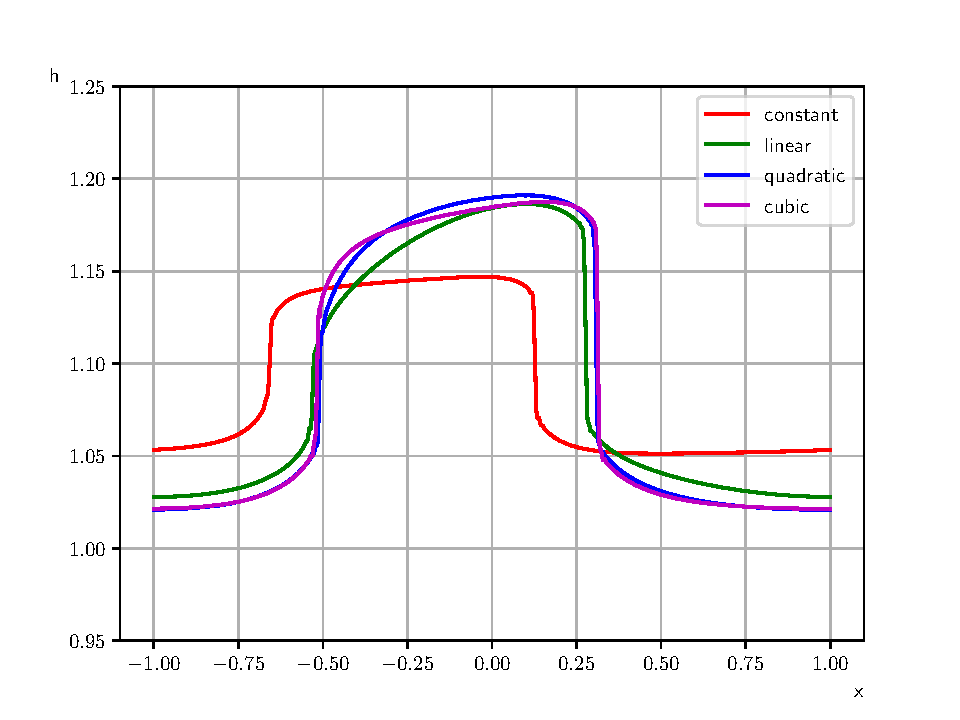
\includegraphics[scale=0.29]{Figures/height_torillhon.pdf}
        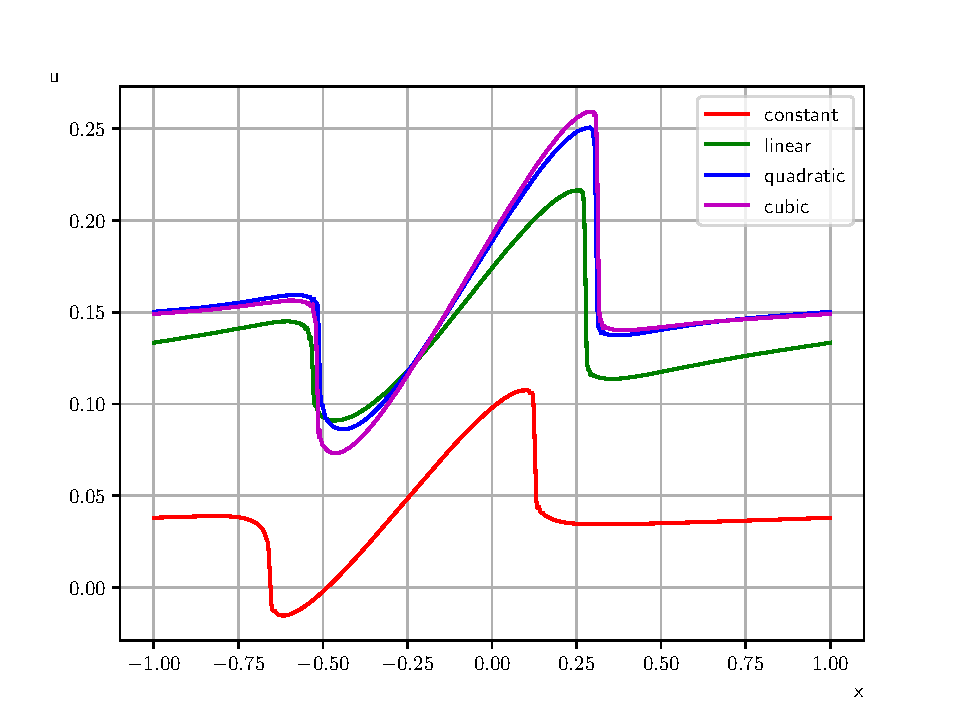
\includegraphics[scale=0.29]{Figures/mean_velocity_torrilhon.pdf}
        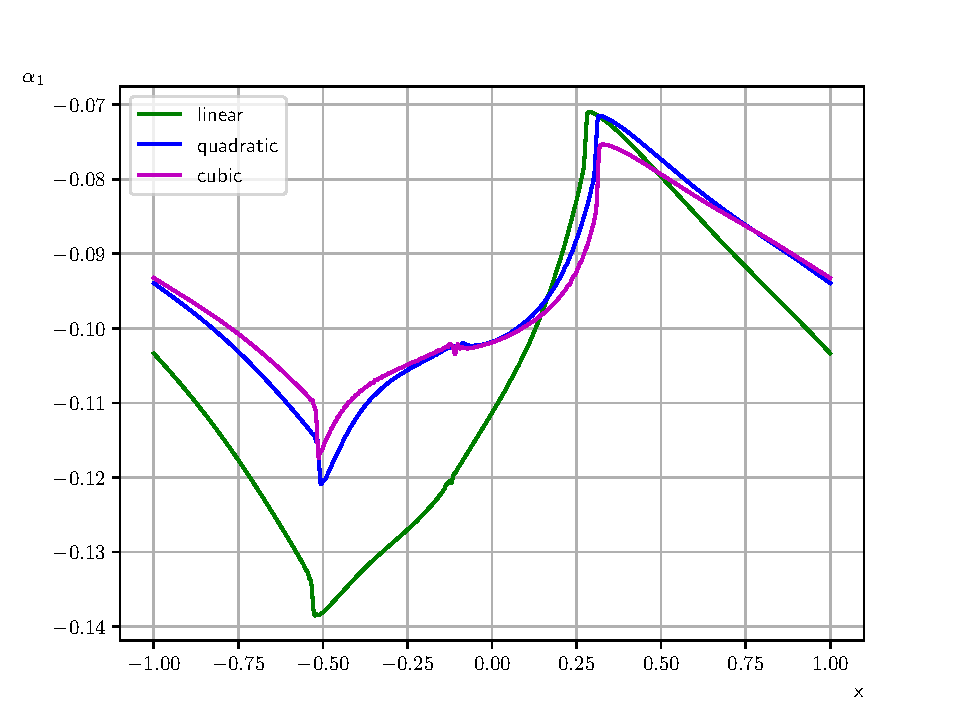
\includegraphics[scale=0.29]{Figures/alpha_1_torrilhon.pdf}
        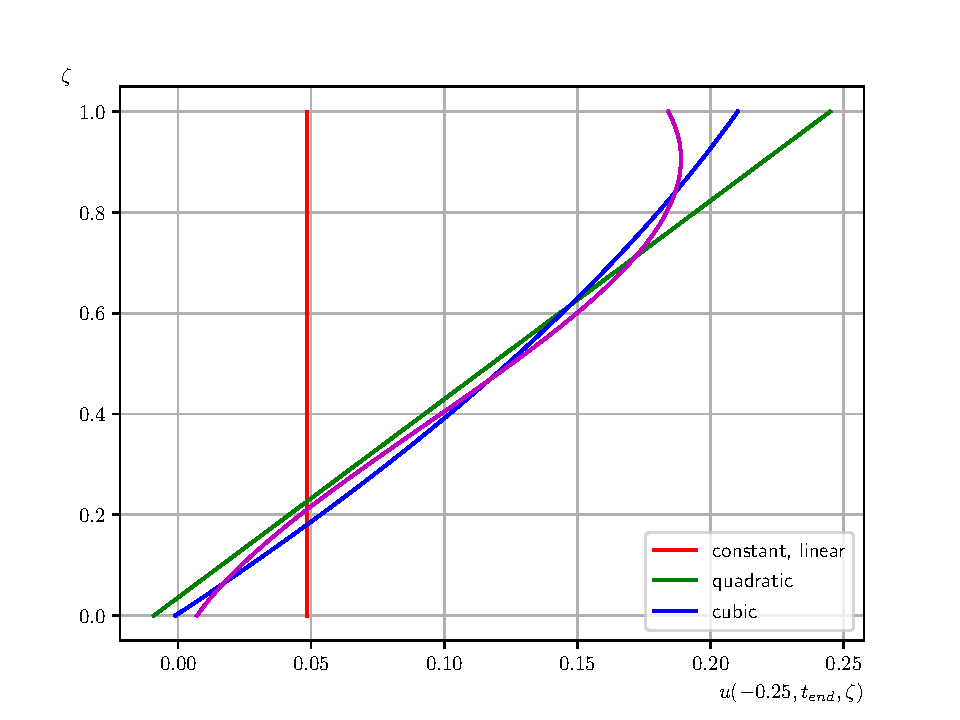
\includegraphics[scale=0.29]{Figures/velocity_profile_-025_torrilhon.pdf}
        % 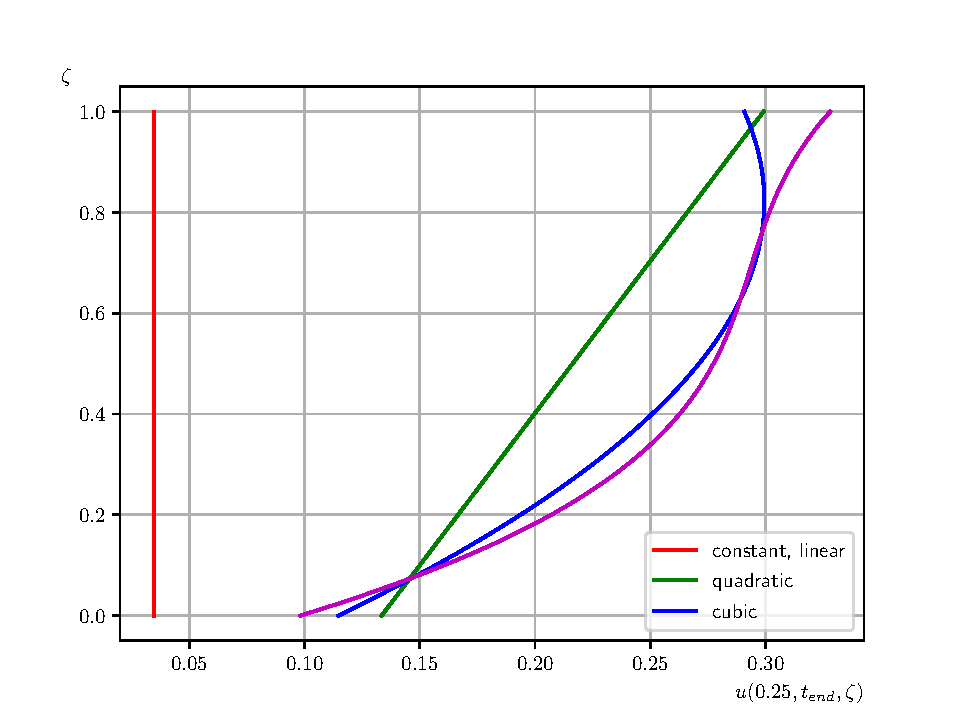
\includegraphics[scale=0.3]{Figures/velocity_profile_025_torrilhon.pdf}
    \end{frame}

    \begin{frame}
        \frametitle{Effect of Higher Moments}
        \centering
        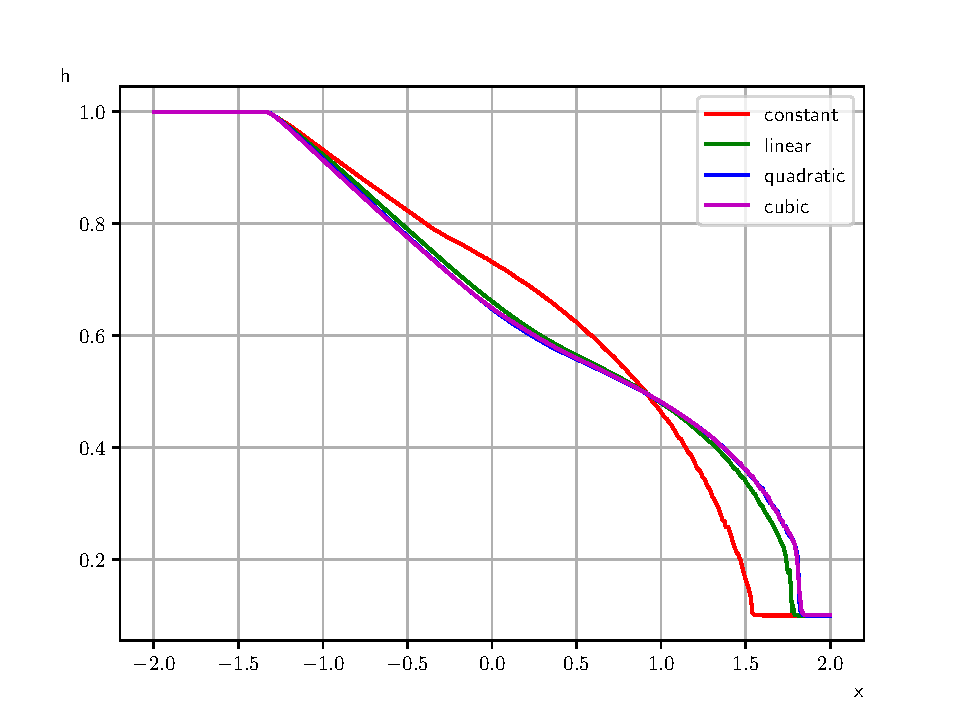
\includegraphics[scale=0.29]{Figures/height_dam.pdf}
        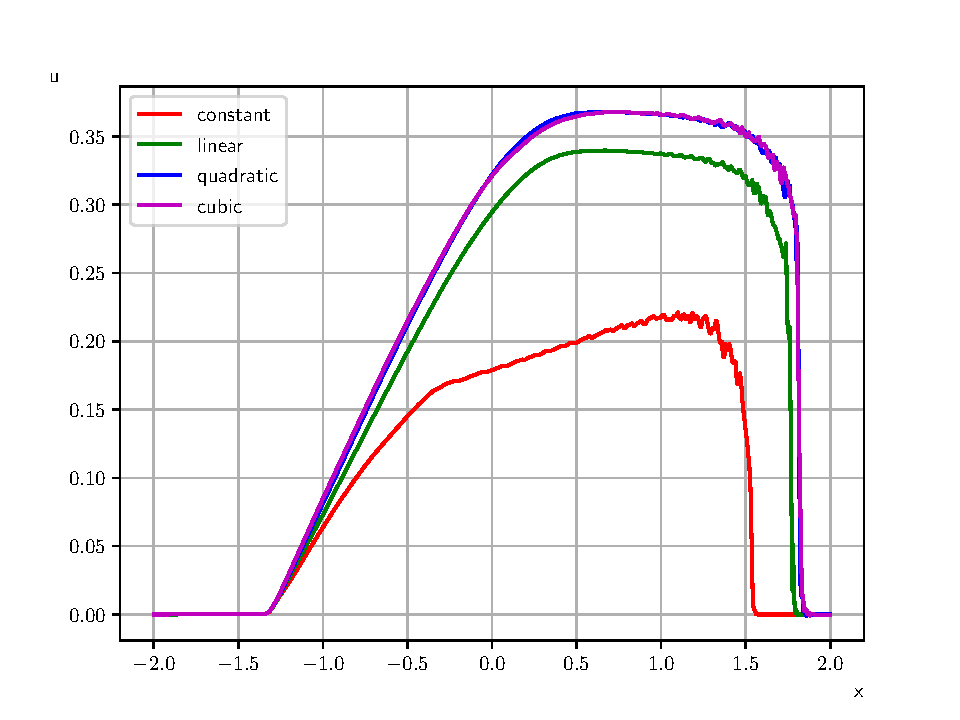
\includegraphics[scale=0.29]{Figures/mean_velocity_dam.pdf}
        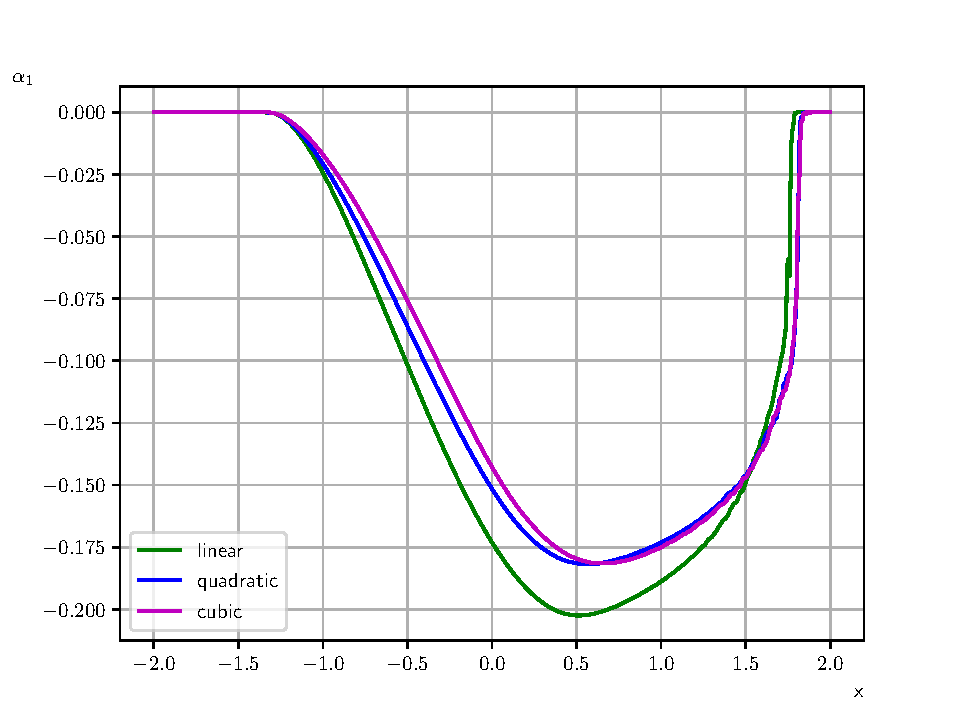
\includegraphics[scale=0.29]{Figures/alpha_1_dam.pdf}
        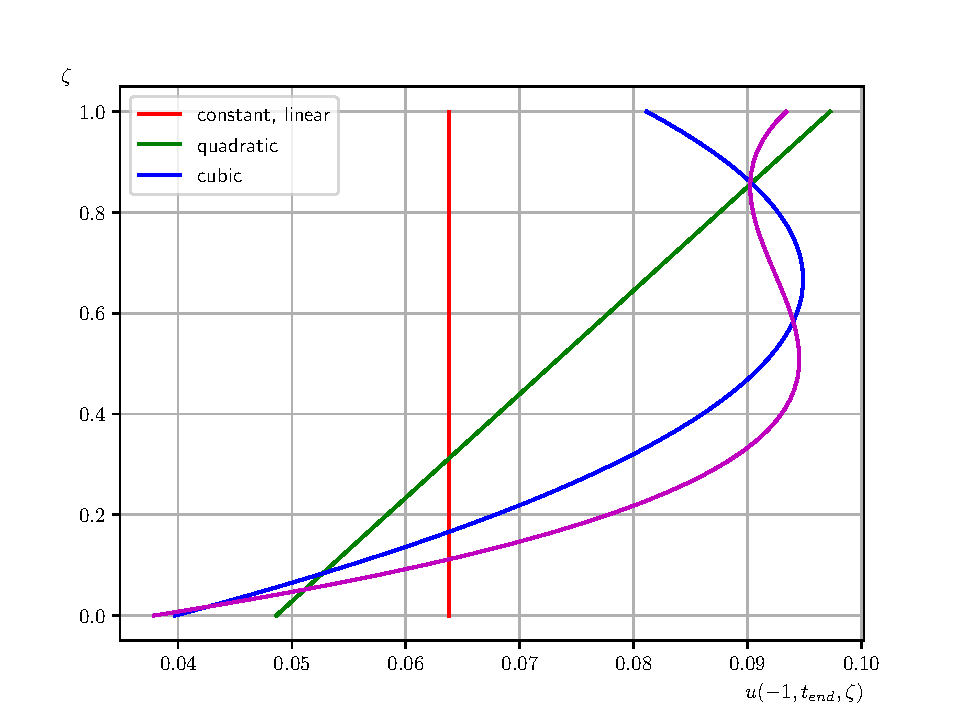
\includegraphics[scale=0.29]{Figures/velocity_profile_-1_dam.pdf}
        % 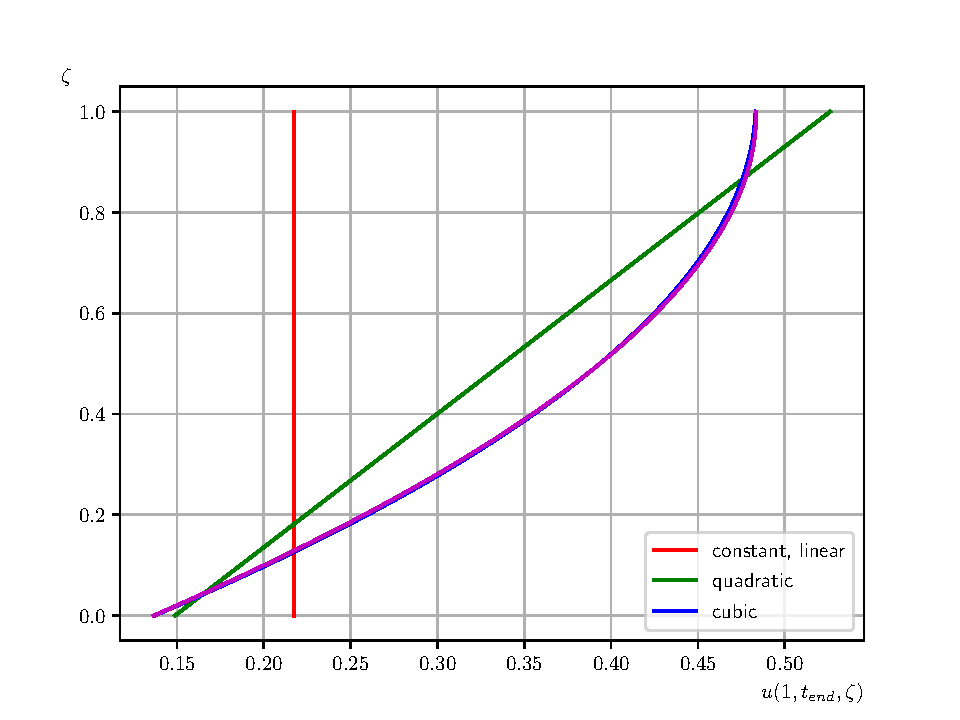
\includegraphics[scale=0.3]{Figures/velocity_profile_1_dam.pdf}
    \end{frame}

    \begin{frame}
      \frametitle{Conclusions}
      Results
      \begin{itemize}
        \item Discontinuous Galerkin Method for Generalized Shallow Water Equations
        \item High Order Method
        \item Properly Discretized Nonconservative Product
      \end{itemize}
      Future Work
      \begin{itemize}
        \item Two Dimensional Meshes
        \item Icosahedral Spherical Mesh
        \item Shallow Water test cases on the sphere
      \end{itemize}

      Supported by SIAM Student Travel Award
    \end{frame}

    \begin{frame}[allowframebreaks]
      \frametitle{Bibliography}
      % TODO: Bibliography
      \nocite{*}
      \printbibliography{}
    \end{frame}

\end{document}
